% Bao cao bai tap lon CS112 - Edit Distance. Bien dich: tectonic -X compile report/report.tex  (hoac Overleaf, XeLaTeX)
% Quy uoc marker:
%   \todo{...}   (do)  = du kien chi nguoi nop biet. Hien khong con cho nao can dien.
%   \verify{...} (cam) = doan do tro ly AI soan tu nhat ky lam viec that; nguoi nop doc va sua cho dung trai nghiem cua minh.
\documentclass[12pt,a4paper]{article}
\usepackage{fontspec}
\setmainfont{Times New Roman}
\setsansfont{Times New Roman}
\setmonofont[Scale=0.88]{Menlo}
\usepackage[vietnamese]{babel}
\usepackage[a4paper,margin=2.5cm]{geometry}
\usepackage{amsmath,amssymb}
\usepackage{xcolor}
\usepackage{graphicx}
\usepackage{booktabs}
\usepackage{longtable}
\usepackage{enumitem}
\usepackage{listings}
\usepackage{hyperref}
\usepackage{float}
\usepackage{caption}
\usepackage{multirow}
\hypersetup{colorlinks=true,linkcolor=black,urlcolor=blue}
\captionsetup{font=small,labelfont=bf}

\newcommand{\todo}[1]{\textcolor{red}{\textbf{[#1]}}}
\newcommand{\verify}[1]{\textcolor{orange!85!black}{\textbf{[XÁC NHẬN: #1]}}}
\newcommand{\code}[1]{\texttt{#1}}

\lstset{basicstyle=\ttfamily\small,columns=fullflexible,keepspaces=true,
  frame=single,framerule=0.3pt,xleftmargin=0.5em,xrightmargin=0.5em,
  breaklines=true,showstringspaces=false}

\begin{document}

% ------------------------------------------------------------------ Bia
\begin{titlepage}
\centering
{\large TRƯỜNG ĐẠI HỌC CÔNG NGHỆ THÔNG TIN, ĐHQG-HCM\par}
\vspace{1.2cm}
{\Large\bfseries BÁO CÁO BÀI TẬP LỚN\par}
{\large Môn: Phân tích và Thiết kế Thuật toán (CS112)\par}
\vspace{1.5cm}
{\LARGE\bfseries TRỰC QUAN HÓA THUẬT TOÁN\\KHOẢNG CÁCH CHỈNH SỬA (EDIT DISTANCE)\par}
\vspace{1.5cm}
\begin{tabular}{ll}
Sinh viên thực hiện: & Đỗ Quốc Hoàng\\
MSSV: & 26410043\\
Lớp: & CS112.F31.LT.TTNT\\
Giảng viên: & Cô Huỳnh Thị Thanh Thương\\
Ngày nộp: & 07/10/2026\\
Mã nguồn: & \url{https://github.com/hoangdq08/uit-edit-distance-visualizer}\\
Video demo: & Nộp kèm file \code{demo.mp4}\\
\end{tabular}
\end{titlepage}

\tableofcontents
\newpage

% ------------------------------------------------------------------ 1
\section{Sản phẩm nộp}
\begin{itemize}[nosep]
  \item \textbf{Source code:} thư mục \code{uit-edit-distance-visualizer/}. Mở \code{index.html} bằng trình duyệt là chạy, không cần cài đặt. Kho mã công khai trên GitHub (liên kết ở trang bìa), bản nộp cũng kèm toàn bộ thư mục.
  \item \textbf{Video demo:} file \code{demo.mp4} nộp kèm, dài 2 phút 26 giây, có giọng đọc.
  \item \textbf{Bộ testcase:} \code{testcases/} (31 test chia 6 nhóm, kèm đáp án và 31 file input).
  \item \textbf{Report:} file này (nguồn LaTeX \code{report/report.tex} và PDF).
\end{itemize}

% ------------------------------------------------------------------ 2
\section{Giới thiệu bài toán}

\textbf{Lý do chọn.} Bài tập Lab\#02 trên Wecode của lớp thuộc chủ đề Quy hoạch động (Dynamic Programming), trong đó có bài ``Rút bài trúng thưởng'' là một bài khoảng cách chỉnh sửa với $n,m\le 5000$. Khi chọn bài cho bài tập lớn, em nhờ AI so sánh ba ứng viên là Edit Distance, Knapsack 0/1 và LIS, rồi chọn Edit Distance theo đề xuất đó. Lý do: bảng quy hoạch động của nó là bảng 2 chiều, mỗi ô chỉ phụ thuộc ba ô lân cận nên rất hợp để trực quan hóa từng bước, và có thêm phần truy vết để ra dãy thao tác cụ thể. Em cũng không chọn hai bài mà cô đã nêu tên trong thông báo (LCS và nhân chuỗi ma trận).

\textbf{Nguồn gốc và ứng dụng.} Khoảng cách này do Levenshtein đưa ra năm 1966 cho mã sửa lỗi \cite{levenshtein}, và cách tính bằng quy hoạch động được trình bày bởi Wagner và Fischer năm 1974 \cite{wagner}. Các ứng dụng quen thuộc: gợi ý sửa lỗi chính tả, các công cụ so sánh tệp (\code{diff}), so khớp chuỗi DNA (dạng tổng quát có trọng số là bài toán gióng hàng chuỗi), và hậu xử lý văn bản sau nhận dạng ký tự.

\textbf{Bài Wecode.} Bản C trong \code{src/edit\_distance.c} (hai hàng, $O(m)$ bộ nhớ) giải bài ``Rút bài trúng thưởng'', được kiểm tra với ví dụ của đề và 600 test ngẫu nhiên đối chiếu với lời giải vét cạn, và được dùng làm một cài đặt đối chứng trong bộ kiểm thử.

% ------------------------------------------------------------------ 3
\section{Mô hình bài toán}
\subsection{Phát biểu}
Cho hai chuỗi $A$ (nguồn) và $B$ (đích). Trên $A$ được phép thực hiện ba loại thao tác, mỗi thao tác tốn một đơn vị: \textbf{thêm} một ký tự, \textbf{xóa} một ký tự, \textbf{thay} một ký tự bằng ký tự khác. Tìm số thao tác \emph{ít nhất} để biến $A$ thành $B$.

\subsection{Mô tả bài toán theo định dạng Wecode}
\textbf{Đề.} Cho hai chuỗi ký tự in hoa. Ta có ba thao tác trên chuỗi thứ nhất: thêm một ký tự, bỏ một ký tự, thay một ký tự bằng ký tự khác. Tìm số thao tác ít nhất để biến chuỗi thứ nhất thành chuỗi thứ hai.

\textbf{Input.} Dòng đầu chứa chuỗi $A$ gồm $n$ ký tự thuộc \code{A..Z}. Dòng thứ hai chứa chuỗi $B$ gồm $m$ ký tự thuộc \code{A..Z}. Ràng buộc $1\le n,m\le 5000$.

\textbf{Output.} Một dòng duy nhất chứa số nguyên $d$ là số thao tác ít nhất.

\begin{center}
\begin{tabular}{@{}ll@{}}
\toprule
Input & Output\\
\midrule
\code{LOVE} & \multirow{2}{*}{2}\\
\code{MOVIE} &\\
\bottomrule
\end{tabular}
\end{center}
\textbf{Giải thích.} Thay \code{L} thành \code{M}, rồi thêm \code{I}.

\subsection{Input và Output}
\begin{center}
\begin{tabular}{@{}llp{8.2cm}@{}}
\toprule
\textbf{Tên} & \textbf{Kiểu} & \textbf{Vai trò và giới hạn}\\
\midrule
$A$ & chuỗi ký tự & chuỗi nguồn, độ dài $n$, ký tự thuộc \code{A..Z}\\
$B$ & chuỗi ký tự & chuỗi đích, độ dài $m$, ký tự thuộc \code{A..Z}\\
$n, m$ & số nguyên & độ dài của $A$, $B$. Giới hạn đề (Wecode): $1\le n,m\le 5000$. Demo: $0\le n,m\le 20$\\
\midrule
$d$ & số nguyên & \textbf{Output}: số thao tác ít nhất, $0\le d\le\max(n,m)$\\
\bottomrule
\end{tabular}
\end{center}
Demo còn in thêm một dãy thao tác cụ thể gồm đúng $d$ bước (không tính các bước ``giữ''). Có thể có nhiều dãy tối ưu, demo chỉ hiển thị một dãy.

\subsection{Ví dụ Input/Output}
\begin{center}
\begin{tabular}{@{}lll@{}}
\toprule
$A$ & $B$ & $d$\\
\midrule
\code{LOVE} & \code{MOVIE} & 2 (thay \code{L} thành \code{M}, thêm \code{I})\\
\code{ABCDEF} & \code{ABCDEF} & 0\\
\code{ABCDEF} & \code{ABCDE} & 1\\
\code{TAT} & \code{TBT} & 1\\
\code{KITTEN} & \code{SITTING} & 3\\
\bottomrule
\end{tabular}
\end{center}

% ------------------------------------------------------------------ 4
\section{Thiết kế thuật toán}
\subsection{Phương pháp vét cạn}
Gọi $f(i,j)$ là số thao tác ít nhất để biến $A[1..i]$ thành $B[1..j]$. Xét ký tự cuối: nếu $A[i]=B[j]$ thì giữ nguyên, ngược lại thử cả ba thao tác. Viết thẳng công thức này thành đệ quy thì mỗi lời gọi sinh ra tối đa 3 lời gọi con, và các bài toán con bị tính lặp rất nhiều lần.

Đếm số lần gọi hàm khi $n=m$: $n=2$ có 19 lời gọi, $n=6$ có 13\,483, $n=10$ có 12\,146\,179 và $n=12$ có 377\,393\,953. Số lời gọi thỏa $T(i,j)=1+T(i-1,j-1)+T(i-1,j)+T(i,j-1)$ nên mỗi lần tăng $n$ thêm 2 thì nhân lên khoảng 25 đến 31 lần ở các cỡ nhỏ, và tỉ lệ này tiến dần tới $(3+2\sqrt2)^2\approx 34$ khi $n$ lớn (tính bằng quy hoạch động trên chính công thức $T$: 32.3 ở $n=20$, 33.1 ở $n=40$). Tức là tăng xấp xỉ $5.83^n$. Thời gian đo được: $n=12$ mất 1.03 giây; ở $n=14$ mất 23.8 giây (đo lại bằng \code{tools/naive\_n14.js}, một lần, kết quả thô ở \code{report/evidence/naive\_n14.json}; một lần đo trước đó trong quá trình làm cho 31.8 giây, nên chênh lệch giữa các lần đo khoảng 30\%). Không thể chạy tới $n=5000$.

\subsection{Cấu trúc dữ liệu}
Bài toán dùng các cấu trúc dữ liệu sau (đặt tên khớp với mã nguồn \code{src/editdistance.js}):
\begin{itemize}[nosep]
  \item \textbf{Hai chuỗi $A$, $B$} lưu dưới dạng mảng ký tự theo điểm mã Unicode (\code{Array.from}), truy cập $A[i]$ trong $O(1)$.
  \item \textbf{Bảng $dp$} kích thước $(n+1)\times(m+1)$, mỗi hàng là một mảng số nguyên 32 bit (\code{Int32Array}). Ô $dp[i][j]$ chỉ phụ thuộc ba ô lân cận $(i-1,j-1)$, $(i-1,j)$, $(i,j-1)$, nên có thể điền theo thứ tự từng hàng. Đây là cấu trúc được hiển thị trực tiếp trên demo.
  \item \textbf{Danh sách bước} (\code{steps}) của demo: một phần tử cho mỗi bước (khởi tạo, mỗi ô, mỗi bước truy vết), mỗi phần tử ghi ô, ba giá trị nguồn và giá trị chọn; giao diện hiển thị trạng thái ứng với chỉ số bước hiện tại, nên Tiến và Lùi là hai thao tác đối xứng.
  \item \textbf{Đường truy vết} là danh sách ô từ $(n,m)$ về $(0,0)$ kèm loại thao tác tại mỗi ô; từ đó suy ra danh sách thao tác theo thứ tự thực hiện.
  \item \textbf{Vì sao giữ cả bảng:} cách truy vết đang cài đặt cần quay lại các ô đã tính nên phải lưu toàn bộ bảng. Bản hai hàng chỉ dùng được khi chỉ cần số $d$.
\end{itemize}
Các lựa chọn khác đã được đo trong thực nghiệm (mục \ref{sec:tn}): đệ quy có nhớ dùng một mảng phẳng $(n+1)(m+1)$ khởi tạo $-1$ để đánh dấu ô chưa tính.

\subsection{Cấu trúc bài toán con và công thức truy hồi}
Chỉ có $(n+1)(m+1)$ cặp $(i,j)$ khác nhau, mỗi cặp chỉ cần tính một lần. Đây là dấu hiệu quy hoạch động.
\begin{align*}
dp[i][0] &= i, \qquad dp[0][j] = j\\
dp[i][j] &= dp[i-1][j-1] \quad\text{nếu } A[i]=B[j]\\
dp[i][j] &= 1+\min\bigl(dp[i-1][j-1],\ dp[i-1][j],\ dp[i][j-1]\bigr) \quad\text{ngược lại}
\end{align*}
trong đó $dp[i-1][j-1]$ ứng với \emph{thay}, $dp[i-1][j]$ ứng với \emph{xóa} $A[i]$, $dp[i][j-1]$ ứng với \emph{thêm} $B[j]$. Đáp án là $d=dp[n][m]$.

\subsection{Mã giả}
\begin{lstlisting}
for i <- 0 to n: dp[i][0] <- i
for j <- 0 to m: dp[0][j] <- j
for i <- 1 to n:
    for j <- 1 to m:
        if A[i] = B[j]:
            dp[i][j] <- dp[i-1][j-1]
        else:
            dp[i][j] <- 1 + min(dp[i-1][j-1], dp[i-1][j], dp[i][j-1])
i <- n; j <- m                       // truy vet
while i > 0 or j > 0:
    if i>0 and j>0 and A[i]=B[j] and dp[i][j]=dp[i-1][j-1]:
        giu A[i]; i <- i-1; j <- j-1
    else if i>0 and j>0 and dp[i][j]=dp[i-1][j-1]+1:
        thay A[i] bang B[j]; i <- i-1; j <- j-1
    else if i>0 and dp[i][j]=dp[i-1][j]+1:
        xoa A[i]; i <- i-1
    else:
        them B[j]; j <- j-1
return dp[n][m]
\end{lstlisting}
Mã giả này trùng với panel ``Mã giả'' trên demo (\code{src/pseudocode.js}): mỗi bước của demo tô sáng đúng các dòng đang thực hiện, và tương ứng này được kiểm thử tự động (mục \ref{sec:tn}).

\subsection{Tính đúng đắn}

Gọi $d(i,j)$ là số thao tác ít nhất (thêm, xóa, thay) để biến $A[1..i]$ thành $B[1..j]$. Chứng minh gồm hai phần: (a) $d(i,j)$ bằng chi phí nhỏ nhất của một \emph{phép gióng hàng} (alignment), (b) $dp[i][j]$ bằng chi phí nhỏ nhất đó, bằng quy nạp theo $i+j$.

\textbf{Phép gióng hàng.} Một phép gióng $A[1..i]$ với $B[1..j]$ là một tập các cặp $(p,q)$ ghép ký tự $A[p]$ với $B[q]$ sao cho các cặp không bắt chéo nhau (nếu $(p,q)$ và $(p',q')$ cùng thuộc tập và $p<p'$ thì $q<q'$). Ký tự của $A$ không được ghép bị \emph{xóa}, ký tự của $B$ không được ghép là ký tự \emph{thêm vào}. Chi phí của phép gióng là số ký tự bị xóa, cộng số ký tự thêm vào, cộng số cặp ghép có hai ký tự khác nhau.

\textbf{(a) Dãy thao tác và phép gióng có cùng chi phí tối thiểu.} Từ một phép gióng ta dựng được dãy thao tác có đúng chi phí đó (xóa các ký tự không ghép, thay các cặp khác nhau, thêm các ký tự còn thiếu). Ngược lại, lấy một dãy thao tác bất kỳ gồm $k$ thao tác và theo dõi từng ký tự gốc của $A$. Các thao tác không làm đổi thứ tự của những ký tự gốc còn tồn tại đến cuối. Ghép mỗi ký tự đó với ký tự mà nó trở thành trong $B$ cho một tập cặp không bắt chéo. Xét chi phí từng loại: mỗi ký tự gốc bị xóa tốn ít nhất 1 thao tác; mỗi ký tự của $B$ không xuất phát từ ký tự gốc nào đã được thêm vào, tốn ít nhất 1 thao tác; mỗi ký tự gốc còn tồn tại nhưng khác ký tự đích đã bị thay ít nhất một lần, tốn ít nhất 1 thao tác; một ký tự được thêm rồi bị xóa tốn ít nhất 2 thao tác mà không tạo chi phí nào trong phép gióng. Cộng lại, chi phí của phép gióng thu được không vượt quá $k$. Vậy $d(i,j)$ chính là chi phí nhỏ nhất của một phép gióng (đây cũng là cách Wagner và Fischer trình bày \cite{wagner}).

\textbf{(b) Cơ sở và công thức truy hồi.} Nếu $i=0$, phải tạo ra $j$ ký tự từ chuỗi rỗng. Mỗi thao tác thêm đúng một ký tự nên cần ít nhất $j$ thao tác và $j$ thao tác là đủ, vậy $d(0,j)=j$. Tương tự $d(i,0)=i$.

Với $i,j>0$, xét một phép gióng tối ưu của $A[1..i]$ với $B[1..j]$ và cặp ký tự cuối $(A[i],B[j])$. Có ba khả năng, bao quát mọi trường hợp:
\begin{enumerate}[nosep]
  \item $B[j]$ không được ghép với ký tự nào của $A$ (là ký tự \emph{thêm vào}): phần còn lại là một phép gióng $A[1..i]$ với $B[1..j-1]$, tổn phí $1+d(i,j-1)$.
  \item $A[i]$ không được ghép với ký tự nào của $B$ (bị \emph{xóa}): phần còn lại gióng $A[1..i-1]$ với $B[1..j]$, tổn phí $1+d(i-1,j)$.
  \item $A[i]$ được ghép đúng với $B[j]$ (giữ nếu bằng nhau, thay nếu khác): phần còn lại gióng $A[1..i-1]$ với $B[1..j-1]$, tổn phí $[A[i]\ne B[j]]+d(i-1,j-1)$.
\end{enumerate}
Ba trường hợp này bao quát mọi phép gióng hàng (một phép gióng có thể thuộc nhiều hơn một trường hợp, điều đó không ảnh hưởng vì ta lấy giá trị nhỏ nhất) vì không có cặp ghép nào bắt chéo: nếu $A[i]$ và $B[j]$ cùng được ghép thì chúng phải ghép với nhau. Phần còn lại trong mỗi trường hợp là một bài toán con cùng dạng nên tối ưu của nó là $d(\cdot,\cdot)$ tương ứng (cấu trúc con tối ưu). Ngược lại, từ một phép gióng tối ưu của bài toán con ta ghép thêm một thao tác để được phép gióng cho $(i,j)$ với đúng tổn phí ở trên, nên $d(i,j)$ không vượt quá cả ba giá trị đó. Vậy $d(i,j)$ bằng giá trị nhỏ nhất của ba tổn phí. Với $A[i]\ne B[j]$ đó chính là công thức thứ ba ở trên.

\textbf{Trường hợp $A[i]=B[j]$ chỉ cần lấy ô chéo.} Khi đó trường hợp 3 có tổn phí $d(i-1,j-1)$. Ta chứng minh nó không lớn hơn hai trường hợp kia. Từ một dãy biến $A[1..i-1]$ thành $B[1..j]$, thêm một thao tác xóa ký tự cuối sẽ được dãy biến $A[1..i-1]$ thành $B[1..j-1]$, nên $d(i-1,j-1)\le 1+d(i-1,j)$. Tương tự, biến $A[1..i-1]$ thành $A[1..i]$ bằng một thao tác thêm rồi áp dụng dãy tối ưu của $(i,j-1)$ cho $d(i-1,j-1)\le 1+d(i,j-1)$. Vậy $\min$ của ba trường hợp bằng $d(i-1,j-1)$.

\textbf{Truy vết.} Mỗi bước đi ngược từ $(i,j)$ chọn một ô trước mà giá trị cộng với chi phí của thao tác tương ứng đúng bằng $dp[i][j]$. Cộng các chi phí dọc đường đi từ $(n,m)$ về $(0,0)$ được $dp[n][m]-dp[0][0]=d$, nên dãy thao tác thu được có đúng $d$ thao tác không phải ``giữ''.

Ngoài chứng minh, tính đúng đắn còn được kiểm tra bằng thực nghiệm (mục \ref{sec:tn}): với mọi testcase, số thao tác không phải ``giữ'' của dãy truy vết bằng $d$ và chuỗi sau thao tác cuối cùng bằng $B$. (Chuỗi này do hàm \code{buildOps} tính từ chính dãy thao tác đó, nên đây là kiểm tra nhất quán chứ không phải một bộ mô phỏng độc lập.)

\subsection{Độ phức tạp}
\begin{center}
\begin{tabular}{@{}lll@{}}
\toprule
Cách cài đặt & Thời gian & Bộ nhớ\\
\midrule
Đệ quy thuần & tăng xấp xỉ $5.83^n$ khi $n=m$ & $O(n+m)$ (ngăn xếp)\\
Đệ quy có nhớ & $O(nm)$ & $O(nm)$\\
Bảng DP (bottom-up) & $O(nm)$ & $O(nm)$\\
DP hai hàng & $O(nm)$ & $O(m)$, \emph{không truy vết được}\\
\bottomrule
\end{tabular}
\end{center}
Truy vết cần giữ cả bảng nên tốn $O(nm)$ bộ nhớ. Với $n=m=5000$ bảng có hơn 25 triệu ô (khoảng 95~MiB nếu mỗi ô 4 byte), còn bản hai hàng chỉ cần khoảng 39~KiB. (Có thuật toán Hirschberg vừa truy vết được vừa chỉ dùng $O(m)$ bộ nhớ, nhưng không được cài trong bài này.)

% ------------------------------------------------------------------ 5
\section{Ứng dụng trực quan hóa}
\subsection{Công nghệ}
HTML, CSS và JavaScript thuần trong một thư mục, mở \code{index.html} là chạy, không cần cài đặt hay máy chủ, không tải font hay thư viện từ mạng. Lõi thuật toán (\code{src/editdistance.js}) dùng chung cho giao diện, bộ kiểm thử và benchmark, nên cái được trình diễn chính là cái được kiểm thử.

\subsection{Chức năng}
\begin{itemize}[nosep]
  \item Nhập hai chuỗi (tối đa 20 ký tự) hoặc chọn ví dụ có sẵn, bấm \emph{Nạp chuỗi}. Demo tự nạp cặp \code{LOVE}$\to$\code{MOVIE} khi mở trang.
  \item \emph{Tiến / Lùi} từng bước, \emph{Tự chạy} (chỉnh tốc độ), \emph{Đầu}, \emph{Kết quả}. Phím tắt: $\rightarrow$, $\leftarrow$, \code{Space}, \code{Home}, \code{End}.
  \item Ba giai đoạn: (1) khởi tạo hàng và cột 0, (2) điền từng ô: tô sáng ô đang tính, ba ô nguồn $\nwarrow\uparrow\leftarrow$ kèm giá trị, ô được chọn viền đậm, công thức cụ thể, (3) truy vết từ ô cuối về $(0,0)$ và hiện dãy thao tác.
  \item Panel mã giả với dòng đang thực hiện được tô vàng, dòng bao quanh (vòng lặp) tô nhạt. Khung Mô hình bài toán nêu Input, Output và công thức truy hồi.
\end{itemize}

\subsection{Ví dụ minh họa các bước thực hiện}
Ví dụ $A=\code{LOVE}$, $B=\code{MOVIE}$. Bảng $dp$ cuối cùng (đường truy vết in đậm):
\begin{center}
\begin{tabular}{c|cccccc}
 & $\varepsilon$ & M & O & V & I & E\\
\hline
$\varepsilon$ & \textbf{0} & 1 & 2 & 3 & 4 & 5\\
L & 1 & \textbf{1} & 2 & 3 & 4 & 5\\
O & 2 & 2 & \textbf{1} & 2 & 3 & 4\\
V & 3 & 3 & 2 & \textbf{1} & \textbf{2} & 3\\
E & 4 & 4 & 3 & 2 & 2 & \textbf{2}\\
\end{tabular}
\end{center}

\textbf{Một ô khác ký tự.} Ô $dp[1][4]$ so $L$ với $I$ (khác nhau): ba nguồn là $dp[0][3]=3$ (thay), $dp[0][4]=4$ (xóa), $dp[1][3]=3$ (thêm), nên $dp[1][4]=1+\min(3,4,3)=4$ (hình~\ref{fig:diff}).

\textbf{Một ô cùng ký tự.} Ô $dp[2][2]$ so $O$ với $O$ (bằng nhau): lấy ô chéo $dp[1][1]=1$ (hình~\ref{fig:same}).

\textbf{Truy vết.} Từ $(4,5)$ qua $(3,4),(3,3),(2,2),(1,1)$ về $(0,0)$, cho dãy thao tác: thay \code{L} thành \code{M} (được \code{MOVE}), giữ \code{O}, giữ \code{V}, thêm \code{I} (được \code{MOVIE}), giữ \code{E}. Tổng 2 thao tác, khớp $dp[4][5]=2$ (hình~\ref{fig:final}). Trạng thái từng bước của cặp này được liệt kê đầy đủ ở phụ lục~\ref{app:steps} (bảng do \code{tools/gen\_steps\_table.js} sinh thẳng từ mô hình mà demo dùng, nên khớp demo từng bước).

\begin{figure}[H]\centering
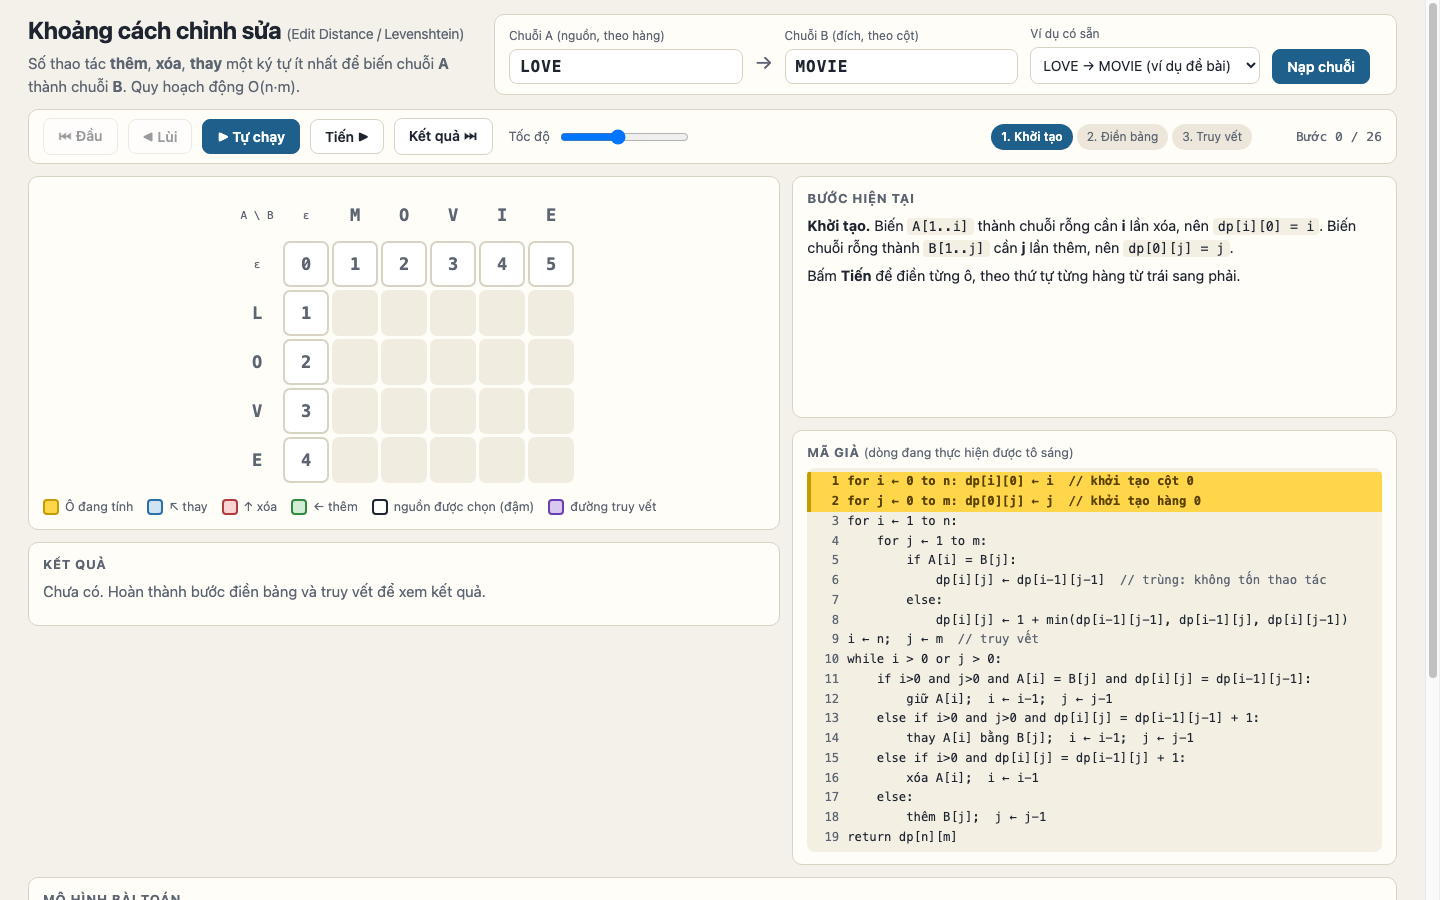
\includegraphics[width=0.96\textwidth]{img/fig1-init.png}
\caption{Bước 0: khởi tạo hàng và cột 0. Bố cục: bảng và kết quả bên trái, giải thích bước và mã giả bên phải.}\label{fig:init}
\end{figure}
\begin{figure}[H]\centering
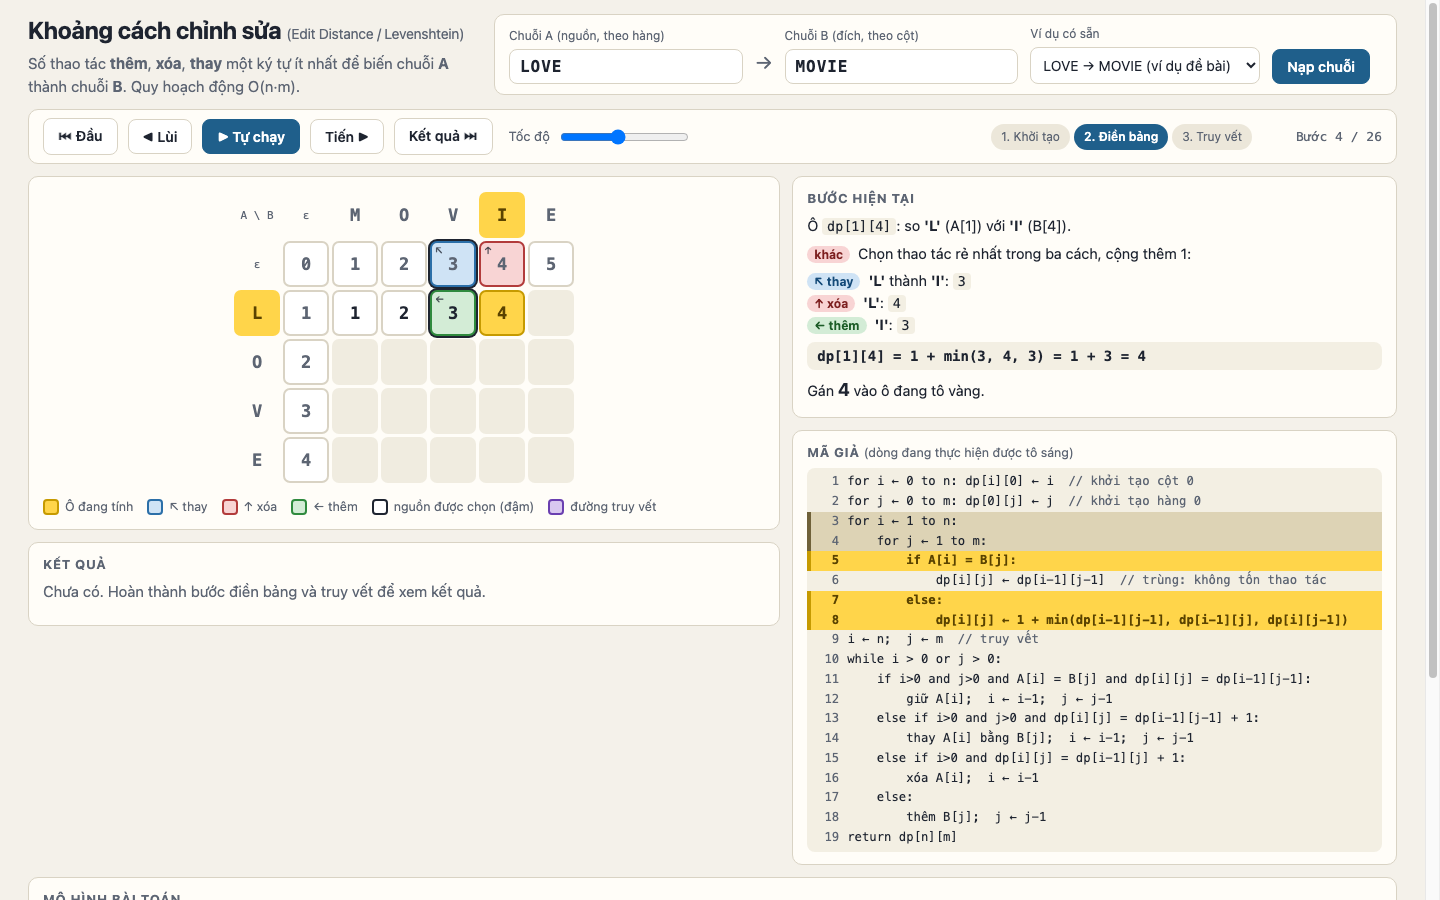
\includegraphics[width=0.96\textwidth]{img/fig3-diff-cell.png}
\caption{Bước 4: ô $dp[1][4]$ khác ký tự. Ba ô nguồn $\nwarrow\uparrow\leftarrow$ được gắn nhãn, ô cho giá trị nhỏ nhất viền đậm; dòng 5, 7, 8 của mã giả sáng.}\label{fig:diff}
\end{figure}
\begin{figure}[H]\centering
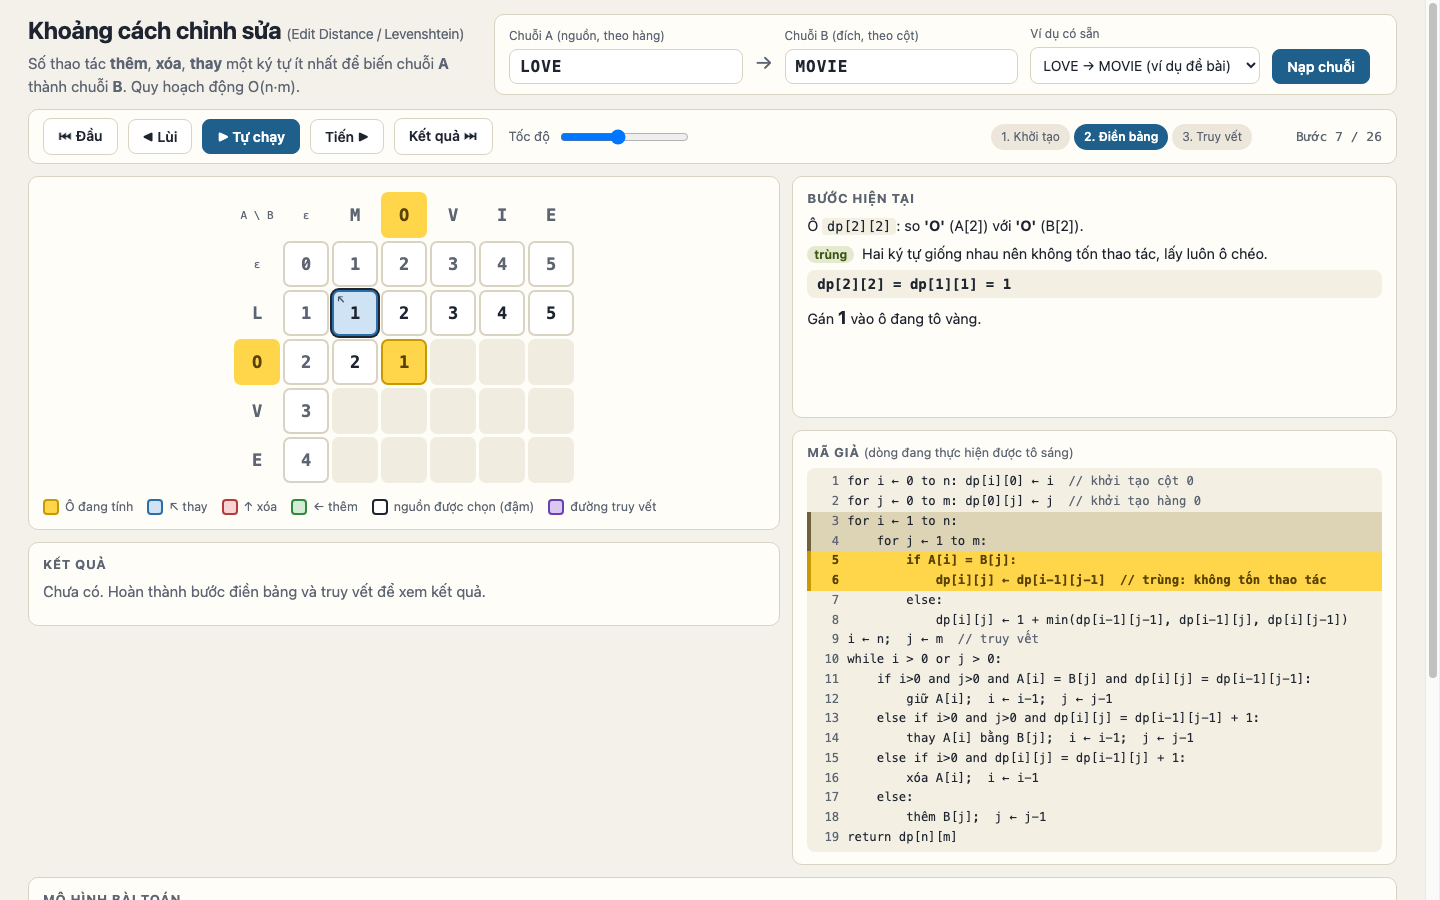
\includegraphics[width=0.96\textwidth]{img/fig2-same-cell.png}
\caption{Bước 7: ô $dp[2][2]$ cùng ký tự. Chỉ có nguồn chéo; dòng 5, 6 của mã giả sáng.}\label{fig:same}
\end{figure}
\begin{figure}[H]\centering
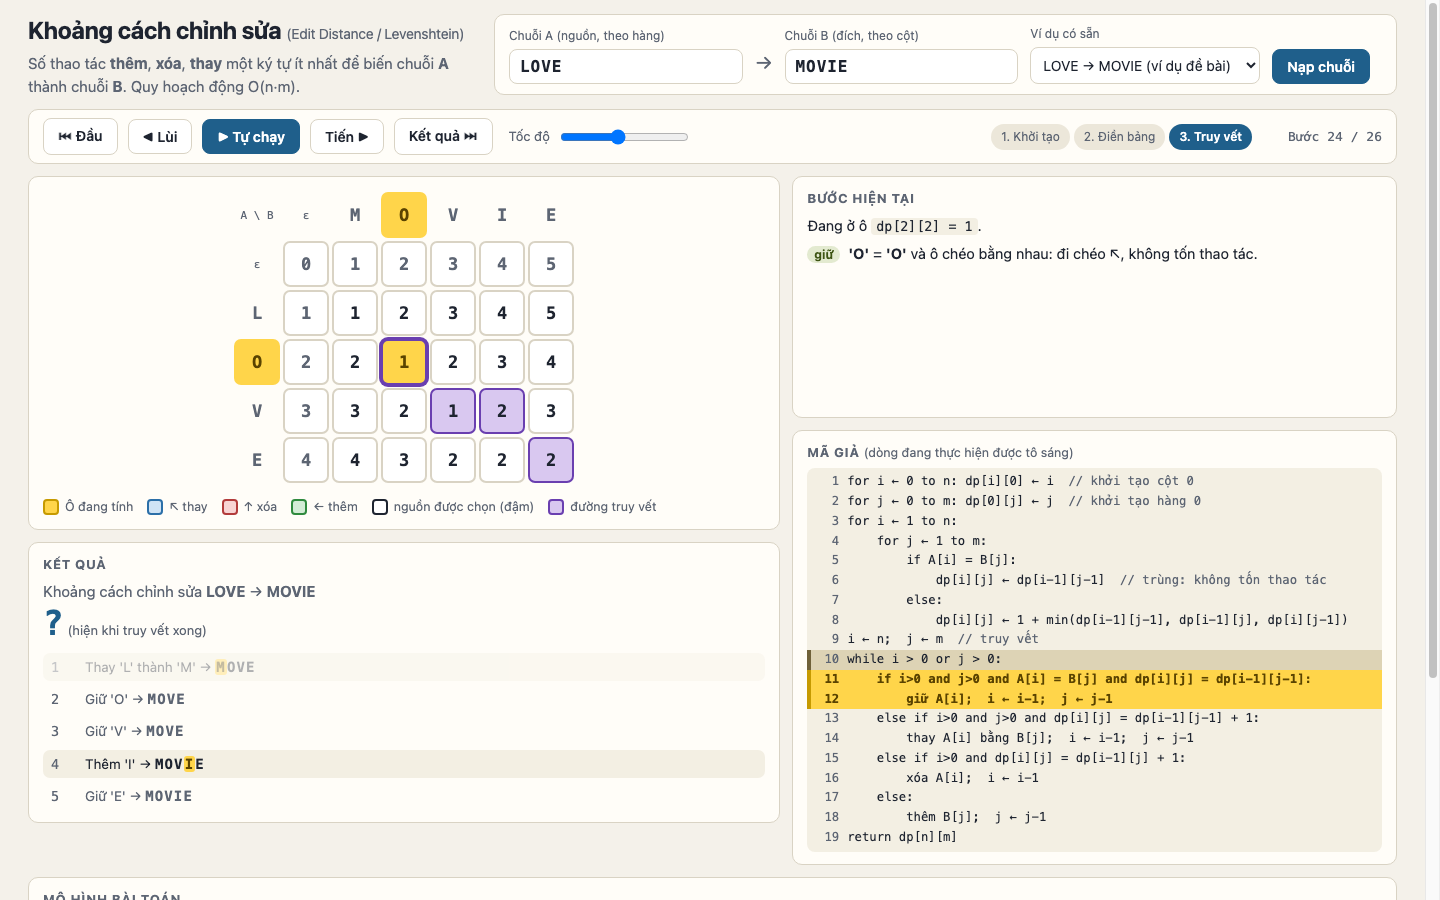
\includegraphics[width=0.96\textwidth]{img/fig4-trace-mid.png}
\caption{Bước 24: đang truy vết. Đường truy vết tô tím, danh sách thao tác lộ dần, đáp án chưa lộ.}\label{fig:trace}
\end{figure}
\begin{figure}[H]\centering
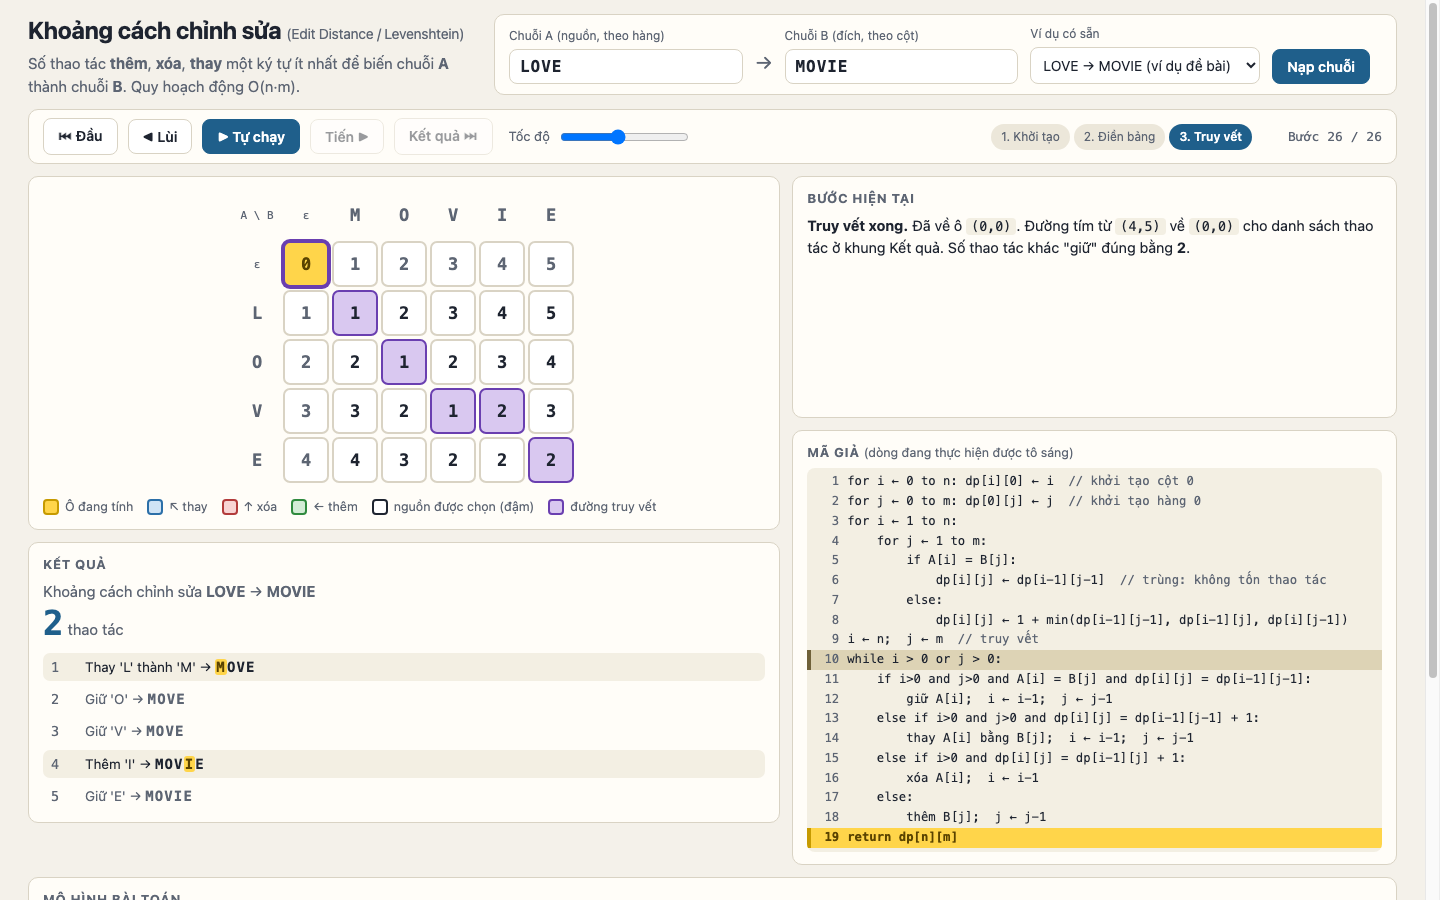
\includegraphics[width=0.96\textwidth]{img/fig5-final.png}
\caption{Bước cuối: đáp án $d=2$ và dãy thao tác kèm chuỗi sau mỗi bước.}\label{fig:final}
\end{figure}

% ------------------------------------------------------------------ 6
\section{Thiết kế thực nghiệm}\label{sec:tn}
\subsection{Cách xây dựng bộ testcase}
Sinh bằng \code{tools/gen\_testcases.py} với hạt giống cố định nên lặp lại được. \textbf{Đáp án (\code{expected}) được tính bằng cài đặt Python độc lập} với bản JavaScript của demo và bản C: DP hai hàng, và với test nhỏ còn đối chiếu thêm với đệ quy có nhớ viết thẳng theo định nghĩa truy hồi. Hai cách phải khớp nhau, nếu không script dừng và không ghi file.

\begin{center}
\begin{tabular}{@{}llp{7.2cm}@{}}
\toprule
\textbf{Nhóm} & \textbf{Số test} & \textbf{Nội dung}\\
\midrule
de-bai & 4 & các ví dụ trong đề (\code{LOVE}/\code{MOVIE}, \code{TAT}/\code{TBT}, \dots)\\
bien & 6 & độ dài 1; một chuỗi là tiền tố, hậu tố hay ở giữa chuỗi kia; đảo chiều để kiểm tra tính đối xứng\\
dac-biet & 8 & khác hoàn toàn, đảo ngược, lặp ký tự, xen kẽ, các ví dụ kinh điển (\code{KITTEN}/\code{SITTING}, \dots)\\
thuong & 5 & ngẫu nhiên, bảng chữ cái nhỏ để có nhiều ký tự trùng\\
lon & 3 & $500\times500$ đến $2000\times2000$\\
gioi-han & 5 & $5000\times5000$: ngẫu nhiên, tất cả khác, giống hệt, một chuỗi dài một chuỗi 1 ký tự, biến thể 50 vị trí\\
\bottomrule
\end{tabular}
\end{center}
Demo giao diện chỉ nhận tối đa 20 ký tự để bảng đọc được, nên \code{tools/run\_tests.js} mới là nơi chạy các test lớn. Demo báo lỗi khi nhập quá 20 ký tự và chấp nhận chuỗi rỗng. Chưa có nhóm kiểm thử cho ký tự ngoài \code{A..Z}.

\subsection{Cách kiểm tra mỗi testcase}
\texttt{node tools/run\_tests.js} kiểm tra, với mỗi testcase:
\begin{enumerate}[nosep]
  \item Cài đặt bảng DP và hai hàng chạy trên \emph{mọi} testcase; đệ quy có nhớ chỉ chạy khi $nm\le 4\,000\,000$ (để không tràn ngăn xếp) và đệ quy thuần chỉ chạy khi $n+m\le 14$ (vì quá chậm). Tất cả đều phải cho đúng đáp án.
  \item Bản C cho đúng đáp án trên cùng input (bước này bị bỏ qua, có thông báo, nếu máy không có \code{gcc}).
  \item Truy vết: số thao tác khác ``giữ'' bằng $d$, và áp dụng các thao tác lên $A$ thì ra đúng $B$.
  \item Đối xứng: $d(A,B)=d(B,A)$.
  \item Ánh xạ mã giả: với mọi bước demo của các cặp cỡ demo, dòng được tô sáng đúng nhánh \code{if/else} và đúng loại thao tác (1377 bước).
\end{enumerate}
Kiểm tra giao diện thật trong trình duyệt: \code{tools/dom\_check.html} chạy trên Chrome headless, đi hết mọi bước của 14 cặp chuỗi (772 bước) và kiểm tra DOM sau mỗi bước (ô đang tính và giá trị, số ô nguồn, dòng mã giả đang sáng, đường truy vết, kết quả không lộ trước khi truy vết xong, trạng thái nút Lùi/Tiến).

\subsection{Kiểm chứng chính bộ kiểm thử}
Để biết bộ kiểm thử có thật sự bắt lỗi, năm lỗi cố ý được chèn vào bản sao của mã giao diện rồi chạy lại (\code{bash tools/mutation\_check.sh}): ánh xạ sai nhánh ``trùng'', ánh xạ sai dòng của thao tác ``xóa'', lộ kết quả sớm, hiện sai giá trị ô, và lộ đáp án qua khung giải thích (lỗi thứ năm do reviewer phát hiện, mục \ref{sec:ai}). Cả năm đều bị báo FAIL, bản gốc báo PASS. Lần chạy đầu chỉ có bốn lỗi và có một đột biến (ánh xạ sai nhánh ``trùng'') vẫn báo PASS, vì kiểm tra so với chính hàm ánh xạ cần kiểm; sau khi sửa, cả năm đột biến đều bị bắt. Chi tiết ở mục \ref{sec:ai}.

% ------------------------------------------------------------------ 7
\section{Đánh giá}
\subsection{Tính đúng đắn}
Kết quả chạy \code{node tools/run\_tests.js}: \textbf{31/31 testcase đạt}, kèm 1377 bước ánh xạ mã giả khớp. Chrome headless: \textbf{PASS, 772 bước, 0 lỗi}.

\subsection{Thời gian thực hiện}
Máy đo: Apple M4, 16~GiB RAM, Node v26.10.0. Chuỗi ngẫu nhiên trên bảng chữ cái 26 ký tự, $n=m$, lấy trung vị của nhiều lần chạy.
\begin{center}
\begin{tabular}{@{}rrrrr@{}}
\toprule
$n=m$ & Đệ quy thuần & Có nhớ & Bảng DP & Hai hàng\\
\midrule
4 & 24.8 $\mu$s & 3.0 $\mu$s & 1.8 $\mu$s & 0.8 $\mu$s\\
8 & 1.08 ms & 1.1 $\mu$s & 0.5 $\mu$s & 0.3 $\mu$s\\
10 & 33 ms & 1.7 $\mu$s & 0.9 $\mu$s & 0.4 $\mu$s\\
12 & 1.03 s & 2.3 $\mu$s & 0.9 $\mu$s & 0.5 $\mu$s\\
100 & -- & 0.15 ms & 43.6 $\mu$s & 17.1 $\mu$s\\
1000 & -- & 18 ms & 3.62 ms & 1.68 ms\\
2000 & -- & 75 ms & 14 ms & 6.68 ms\\
5000 & -- & 472 ms & 87 ms & 42 ms\\
\bottomrule
\end{tabular}
\end{center}
Đệ quy thuần không chạy tiếp từ $n=14$ vì mất hơn 20 giây (xem mục 4.1). Từ $n=1000$ lên $n=5000$ tích $nm$ tăng 25 lần, thời gian của bảng DP tăng từ 3.62 ms lên 87 ms, tức 24 lần, khớp với $O(nm)$. Ở $n=5000$, đệ quy có nhớ chậm hơn bảng DP 5.4 lần và bảng DP chậm hơn bản hai hàng 2.1 lần. Chênh lệch này có thể do chi phí gọi hàm và cách truy cập bộ nhớ (bảng đầy đủ gần 95~MiB, bản hai hàng nhỏ hơn nhiều); em chưa đo riêng nguyên nhân. Bản C (\code{gcc -O2}, $n=5000$) chạy trong 14~ms tính cả khởi động tiến trình, nên không so trực tiếp với các cột trên. Số liệu thô nằm ở \code{testcases/benchmark\_result.json}.

\subsection{Hạn chế}
\begin{itemize}[nosep]
  \item Demo chỉ nhận tối đa 20 ký tự mỗi chuỗi. Thuật toán chạy tới 5000 ký tự nhưng không có giao diện từng bước ở cỡ đó.
  \item Truy vết chọn một đường tối ưu theo thứ tự ưu tiên giữ/thay, xóa, thêm, dù có thể có nhiều đường cùng số thao tác.
  \item Đệ quy có nhớ sâu $n+m$ nên có thể tràn ngăn xếp với chuỗi rất dài.
  \item Bảng 20$\times$20 có ô nhỏ (khoảng 28~px ở màn hình 1440~px) nên nhãn mũi tên nguồn rất nhỏ; khung Kết quả nằm dưới bảng nên với bảng này phải cuộn mới thấy.
  \item Ở màn hình hẹp (1100~px) bố cục thành một cột và mã giả phải cuộn mới thấy.
  \item Hướng phát triển: khoảng cách Damerau (thêm phép hoán vị hai ký tự kề nhau), trọng số khác nhau cho từng thao tác, thuật toán Hirschberg để vừa truy vết vừa chỉ dùng $O(m)$ bộ nhớ.
\end{itemize}

% ------------------------------------------------------------------ 8
\section{Quy trình thực hiện với AI}\label{sec:ai}

\subsection{Công cụ}
\begin{itemize}[nosep]
  \item Em dùng \textbf{Jcode} (trợ lý lập trình trên dòng lệnh) làm công cụ chính. Model điều phối trong phiên: Claude Sonnet 5.5.
  \item Em dùng \textbf{GPT-6-sol} (khác họ model với Claude) để đánh giá độc lập kết quả của AI. GPT chỉ đọc, không được sửa tệp; em dựa vào đánh giá đó để yêu cầu sửa.
  \item Chrome headless (kiểm tra DOM, chụp ảnh), Node, gcc, Python, \code{tectonic} (biên dịch LaTeX).
\end{itemize}

\subsection{Phân công}
\textbf{Em thực hiện:} em chọn bài toán Edit Distance theo yêu cầu của cô, quyết định làm demo trên web, đặt từng yêu cầu cho AI theo các prompt ở mục 8.3, xem kết quả sau mỗi lần và yêu cầu sửa những chỗ chưa đúng (các lỗi ở mục 8.4). Em cũng dùng GPT-6-sol để đánh giá độc lập, và quyết định nội dung giữ hoặc bỏ trong báo cáo.

\textbf{AI hỗ trợ:} AI được dùng như công cụ để cài đặt (mã nguồn, mã giả, bộ kiểm thử, benchmark, bản C), sinh testcase và đáp án đối chứng, và soạn nội dung báo cáo từ dữ liệu chạy thật. Công thức truy hồi là thuật toán chuẩn trong giáo trình (Wagner--Fischer), do AI đề xuất khi em chọn bài, không phải do em phát minh.

\subsection{Quá trình tìm hiểu, các bước và prompt chính}
\textbf{Quá trình tìm hiểu và chọn hướng.} Em làm theo thứ tự sau.
\begin{enumerate}[nosep]
  \item \emph{Đọc yêu cầu của cô.} Em đưa trang giao bài trên Moodle cho AI đọc để xác định cần nộp gì: demo có giao diện nhập Input, theo dõi từng bước và xem Output, bộ testcase, video và report. Em lấy các yêu cầu này làm tiêu chí xuyên suốt, và để ý cô đã nêu tên hai bài (LCS, nhân chuỗi ma trận) nên em không chọn hai bài đó.
  \item \emph{Chọn bài toán.} Em hỏi AI đề xuất bài cho bài tập lớn. AI so sánh Edit Distance, Knapsack 0/1 và LIS. Em đối chiếu với yêu cầu của cô và chọn Edit Distance vì bảng quy hoạch động là bảng 2 chiều, mỗi ô chỉ phụ thuộc ba ô lân cận, rất hợp để minh họa từng bước, và có thêm phần truy vết ra dãy thao tác. Bài ``Rút bài trúng thưởng'' trong Lab\#02 là một bài cùng dạng nên em cũng có sẵn đề và giới hạn $n,m\le 5000$ để làm chuẩn.
  \item \emph{Chọn hình thức.} Em hỏi nên viết thành ứng dụng riêng hay web, nghe phân tích và chọn web một thư mục để người chấm chỉ cần mở \code{index.html}.
  \item \emph{Đánh giá bằng GPT.} Sau khi có bản đầu, em hỏi có nên dùng GPT để đánh giá lại không và chọn chạy. GPT-6-sol (khác họ model với Claude) đánh giá độc lập, chỉ đọc; em yêu cầu sửa theo các điểm nó chỉ ra. Về sau em yêu cầu thêm các lượt đánh giá bằng GPT-6-sol để kiểm tra số liệu, đối chiếu yêu cầu của cô và chỉnh văn phong, tính hợp lý của báo cáo.
\end{enumerate}

\textbf{Các bước và prompt.} Trong ngoặc kép là câu em đã gõ thật trong cuộc trò chuyện (ngày 07/10/2026), rút gọn nếu dài. Mỗi dòng đi từ việc em yêu cầu, đến việc em quyết định, rồi kết quả AI trả.
\begin{center}
\small
\begin{tabular}{@{}p{0.4cm}p{5.0cm}p{5.4cm}p{3.4cm}@{}}
\toprule
\# & Em yêu cầu & Em quyết định hoặc làm tiếp & AI trả\\
\midrule
1 & Gửi đề Wecode, yêu cầu viết bằng C: \emph{``dùng ngôn ngữ c để viết''} & Dùng bản C để đối chiếu với các cài đặt khác & Lời giải $O(n\cdot m)$, bộ nhớ hai hàng\\
2 & Đưa trang giao bài của cô: \emph{``đọc link này đi''} & Lấy yêu cầu của cô làm căn cứ cho các bước sau & Tóm tắt yêu cầu bài tập lớn\\
3 & Hỏi chọn bài cho bài tập lớn: \emph{``đề xuất sao''} & Em chọn Edit Distance & So sánh Edit Distance, Knapsack, LIS\\
4 & Hỏi \emph{``có nên viết dưới dạng app chạy thay vì web không''} & Em chọn web & Nên giữ web một thư mục\\
5 & Hỏi \emph{``có cần dùng gpt để đánh giá lại không''}, rồi \emph{``chạy đi''} & Chọn dùng GPT để đánh giá, yêu cầu sửa các điểm nó chỉ ra & GPT-6-sol đánh giá độc lập (chỉ đọc)\\
6 & \emph{``làm khung report''}; sau đó yêu cầu kiểm tra: \emph{``tôi kiểm tra lại, có thể thêm swarm để review, kiểm tra, đánh giá''} & Yêu cầu sửa các lỗi 8 và 9 ở mục 8.4 (lỗi 6, 7 lộ ra khi đối chiếu số liệu) & Dựng khung report; GPT-6-sol kiểm tra số liệu và đối chiếu yêu cầu của cô\\
7 & \emph{``điều chỉnh lại văn phong, tính hợp lý, chuẩn theo yêu cầu của cô''} & Yêu cầu sửa các chỗ GPT chỉ ra & GPT-6-sol đánh giá văn phong, chỉ ra tham chiếu sai, chỗ thừa\\
\bottomrule
\end{tabular}
\end{center}

\subsection{Lỗi gặp phải và cách phát hiện, sửa}
Các lỗi sau là lỗi em gặp thật sau các lần prompt: khi AI trả kết quả, lỗi xuất hiện và em yêu cầu AI sửa. Cột ``Phát hiện bằng'' ghi công cụ hoặc reviewer đã cho thấy lỗi (trình biên dịch, lệnh chạy, ảnh chụp giao diện, trợ lý AI hoặc reviewer). Lỗi 6, 7 và 9 là lỗi của chính bản nháp report, lộ ra khi đối chiếu với số liệu thật hoặc nhờ reviewer.
{\small
\begin{longtable}{@{}p{0.4cm}p{5.1cm}p{4.2cm}p{4.3cm}@{}}
\toprule
\# & Lỗi gặp phải & Phát hiện bằng & Cách sửa\\
\midrule
\endhead
1 & Code C hoán đổi hai hàng bằng cách gán mảng (\code{tmp = prev; prev = cur}), không biên dịch được & Trình biên dịch báo ``array type is not assignable'' & Dùng con trỏ \code{int *prev, *cur}\\
2 & Test chạy cả testcase 5000$\times$5000 qua hàm tạo mô hình từng bước, hết bộ nhớ (hơn 4~GB) & Node thoát với lỗi hết heap & Test truy vết dùng hàm riêng; chỉ demo mới dùng mô hình từng bước (giới hạn 20 ký tự)\\
3 & Benchmark treo 5 phút vì để đệ quy thuần chạy tới $n=20$ & Lệnh chạy quá thời gian 300 giây & Chỉ chạy đệ quy thuần tới $n=12$, ghi rõ lý do trong mã\\
4 & Chạy mutation test lần đầu không in ra kết quả nào, vì bộ lọc output của lệnh sai, nên chưa kết luận được gì & Thấy cả ba lần chạy đều trống, kể cả bản gốc & Sửa bộ lọc, chạy lại\\
5 & Kiểm tra DOM chỉ so sánh với chính hàm ánh xạ mã giả, nên một lỗi ánh xạ nhánh ``trùng'' lọt qua (báo PASS khi đã chèn lỗi) & Chạy lại sau khi sửa bộ lọc, thấy đúng một đột biến vẫn PASS & Đọc chữ thật của dòng đang sáng trên trang để so; chạy lại: 4/4 lỗi bị bắt (về sau thêm lỗi thứ năm, lỗi 8 ở bảng này)\\
6 & Bản nháp report ghi ``nhân khoảng 30 lần'' và ``$\Theta(5.83^n)$'', chưa đúng với số đo & Tính lại số lời gọi bằng quy hoạch động: 25 đến 31 ở cỡ nhỏ, tiến dần tới 34 & Viết lại cho khớp số đo\\
7 & Bản nháp ghi bản C là ``đã nộp lên Wecode'' khi không có bằng chứng nộp & Đối chiếu lại nhật ký làm việc & Đổi thành ``giải bài Wecode'', không khẳng định đã nộp\\
8 & Đáp án vẫn lộ ở câu ``đây là kết quả: $d$'' của bước truy vết đầu, dù khung Kết quả đã ẩn; bộ kiểm tra DOM chỉ nhìn khung Kết quả nên bỏ sót & Reviewer GPT-6-sol; đã tái hiện trong Chrome (bước 21 có ``kết quả:'' khi \code{\#result} vẫn là ``?'') & Xóa câu đó; thêm kiểm tra khung giải thích vào DOM check và thêm đột biến thứ năm (bị bắt)\\
9 & Chứng minh tính đúng đắn bản đầu chia mọi dãy tối ưu thành ba trường hợp theo ký tự cuối mà không nêu bước chuẩn hóa về phép gióng hàng & Reviewer GPT-6-sol (hai bất đẳng thức phụ đúng, chỉ thiếu bước này) & Viết lại mục 4.5 theo phép gióng hàng, dẫn Wagner--Fischer\\
\bottomrule
\end{longtable}
}

\subsection{Nhận xét}
Nhìn lại các lỗi ở bảng trên, đa số là lỗi khó nhận ra nếu chỉ nhìn kết quả ban đầu: một bộ kiểm thử báo PASS khi đã chèn lỗi, đáp án vẫn lộ ở một đoạn lời giải thích trong khi khung Kết quả đã ẩn, chứng minh thiếu một bước chuẩn hóa, và hai số đo ghi sai trong bản nháp. Tất cả chỉ lộ ra khi chạy lại, đối chiếu với số thật hoặc nhờ một reviewer khác họ model.

Về thuật toán, điều em rút ra là bảng quy hoạch động đủ để tìm số thao tác ít nhất vì mỗi ô chỉ phụ thuộc ba ô lân cận, và dãy thao tác cụ thể được lấy lại bằng cách truy vết ngược từ ô cuối. Về việc dùng AI, em rút ra là không nên coi một kết quả báo đạt là đủ khi chưa có cách kiểm tra độc lập với chính phần được kiểm tra.


% ------------------------------------------------------------------ 9
\section{Kết luận}
Bài tập lớn trực quan hóa thuật toán khoảng cách chỉnh sửa bằng quy hoạch động $O(nm)$: demo web từng bước (khởi tạo, điền bảng, truy vết) kèm mã giả tô sáng dòng đang chạy, bộ 31 testcase với đáp án tính độc lập, và benchmark so bốn cách cài đặt. Cả 31 testcase đạt, kiểm tra giao diện trên Chrome đạt 772 bước và kiểm tra bằng đột biến bắt được cả 5 lỗi chèn vào. Đệ quy thuần tăng xấp xỉ $5.83^n$ và không dùng được quá $n\approx 12$, trong khi quy hoạch động chạy $n=m=5000$ trong 87 ms (bảng đầy đủ). Hạn chế chính là demo chỉ nhận 20 ký tự và khung Kết quả bị đẩy xuống dưới với bảng lớn.

\begin{thebibliography}{9}
\bibitem{levenshtein} V. I. Levenshtein, ``Binary codes capable of correcting deletions, insertions and reversals'', \emph{Soviet Physics Doklady}, 10(8), 707--710, 1966.
\bibitem{wagner} R. A. Wagner, M. J. Fischer, ``The string-to-string correction problem'', \emph{Journal of the ACM}, 21(1), 168--173, 1974.
\bibitem{cormen} T. H. Cormen, C. E. Leiserson, R. L. Rivest, C. Stein, \emph{Introduction to Algorithms}, chương Dynamic Programming, MIT Press.
\end{thebibliography}

\appendix
\section{Trạng thái từng bước của ví dụ \code{LOVE} $\to$ \code{MOVIE}}\label{app:steps}
Bảng dưới đây liệt kê mọi bước của demo (26 bước sau bước 0). Cột $\nwarrow,\uparrow,\leftarrow$ là ba giá trị nguồn; khi hai ký tự trùng chỉ dùng nguồn chéo. Sinh bằng \code{node tools/gen\_steps\_table.js LOVE MOVIE}. Bảng thứ hai là các bước truy vết, đi ngược từ ô cuối $(4,5)$ về $(0,0)$, nên thao tác thay \code{L} thành \code{M} xuất hiện ở cuối bảng; khi áp dụng lên $A$ theo thứ tự thực hiện (từ trái sang phải) thì thao tác này đứng đầu, như trong danh sách ở mục 5.3.
\begin{center}\small
\begin{tabular}{@{}rcclrrrr@{}}
\toprule
Bước & Ô & $A[i]$ vs $B[j]$ & Nhánh & $\nwarrow$ & $\uparrow$ & $\leftarrow$ & Giá trị\\
\midrule
0 & \multicolumn{7}{l}{khởi tạo hàng và cột 0: $dp[i][0]=i$, $dp[0][j]=j$}\\
1 & (1,1) & \code{L} / \code{M} & min & 0 & 1 & 1 & \textbf{1}\\
2 & (1,2) & \code{L} / \code{O} & min & 1 & 2 & 1 & \textbf{2}\\
3 & (1,3) & \code{L} / \code{V} & min & 2 & 3 & 2 & \textbf{3}\\
4 & (1,4) & \code{L} / \code{I} & min & 3 & 4 & 3 & \textbf{4}\\
5 & (1,5) & \code{L} / \code{E} & min & 4 & 5 & 4 & \textbf{5}\\
6 & (2,1) & \code{O} / \code{M} & min & 1 & 1 & 2 & \textbf{2}\\
7 & (2,2) & \code{O} / \code{O} & trùng & 1 & -- & -- & \textbf{1}\\
8 & (2,3) & \code{O} / \code{V} & min & 2 & 3 & 1 & \textbf{2}\\
9 & (2,4) & \code{O} / \code{I} & min & 3 & 4 & 2 & \textbf{3}\\
10 & (2,5) & \code{O} / \code{E} & min & 4 & 5 & 3 & \textbf{4}\\
11 & (3,1) & \code{V} / \code{M} & min & 2 & 2 & 3 & \textbf{3}\\
12 & (3,2) & \code{V} / \code{O} & min & 2 & 1 & 3 & \textbf{2}\\
13 & (3,3) & \code{V} / \code{V} & trùng & 1 & -- & -- & \textbf{1}\\
14 & (3,4) & \code{V} / \code{I} & min & 2 & 3 & 1 & \textbf{2}\\
15 & (3,5) & \code{V} / \code{E} & min & 3 & 4 & 2 & \textbf{3}\\
16 & (4,1) & \code{E} / \code{M} & min & 3 & 3 & 4 & \textbf{4}\\
17 & (4,2) & \code{E} / \code{O} & min & 3 & 2 & 4 & \textbf{3}\\
18 & (4,3) & \code{E} / \code{V} & min & 2 & 1 & 3 & \textbf{2}\\
19 & (4,4) & \code{E} / \code{I} & min & 1 & 2 & 2 & \textbf{2}\\
20 & (4,5) & \code{E} / \code{E} & trùng & 2 & -- & -- & \textbf{2}\\
\bottomrule
\end{tabular}
\end{center}

% --- truy vet (di nguoc tu o cuoi ve (0,0)) ---
\begin{center}\small
\begin{tabular}{@{}rcll@{}}
\toprule
Bước & Ô & Thao tác & Giá trị ô\\
\midrule
21 & (4,5) & giữ \code{E} & 2\\
22 & (3,4) & thêm \code{I} & 2\\
23 & (3,3) & giữ \code{V} & 1\\
24 & (2,2) & giữ \code{O} & 1\\
25 & (1,1) & thay \code{L} thành \code{M} & 1\\
26 & (0,0) & xong, về $(0,0)$ & 0\\
\bottomrule
\end{tabular}
\end{center}


\section{Hướng dẫn chạy}
\begin{lstlisting}
# demo: mo index.html bang trinh duyet
python3 tools/gen_testcases.py   # sinh lai testcase (can Python 3)
node tools/run_tests.js          # can Node, gcc de kiem tra ban C
node tools/benchmark.js          # khoang 10 giay
# chup lai anh minh hoa (tool/shot.html), kiem tra DOM (tools/dom_check.html): xem README.md
\end{lstlisting}

\end{document}
